\section{External-validity evidence}
\label{sec:external}
The external-validity study (V4 in the artifacts) tests alternative target
rules (W1), a second model family (W2), and a second arrival source (W4) under
the same deadline and cost definitions. Each test is evaluated separately. The tables distinguish technical
validity from strict qualification: the latter keeps the original request
denominator, requires at least 99\% online on-time completion, every offline
job timely, and all requests completed without unfinished or censored work.
A late offline completion is not an unfinished request, but neither qualifies.
Table~\ref{tab:coverage} accounts for all 93 original V4 identities, including gates
and six historical reuses. E1 adds 14 separately accounted formal identities
(Section~\ref{app:e1}); requests are not independent experimental repeats.

\subsection{Alternative unguarded target rules}
The alternative-controller test (W1) asks whether unguarded rules can also
complete all work on time. B-HPA is an HPA-inspired queue-target controller with a
stabilization interval, not an implementation of Kubernetes HPA. B-PRED applies a
causal Holt queue predictor; B-MMC selects a capacity from the past arrival-rate
estimate and the frozen E service lookup. The three policies share the two-instance
limit, lifecycle semantics, one-second observation tick, and 60-second action
cooldown. None uses the V3 deadline guard, observes future arrivals, or trains a
learned scheduler. No registered development candidate qualified, so all three
use their predeclared center fallback; they are not presented as optimized
best-in-family implementations. Section~\ref{app:baselinecontract} records their
grids, locks, and semantic validation.

All three baselines complete all nine formal runs with timely online and offline
work (Table~\ref{tab:w1}). Their equal-window scenario costs are 2.2305, 4.0085,
and 2.7861, respectively. Each exceeds the historical V3 all1 reference, showing that timely completion
alone does not identify the lowest-cost policy. All three succeed without the
guard; adding the guard to these controllers remains untested. B-PRED's per-run online p99 is 1.58--2.70 seconds across these windows,
whereas B-HPA and B-MMC reach 15--19 seconds in steady/recovery. Thus the
higher-cost predictor also exposes a latency--resource trade-off;
Table~\ref{tab:w1latency} reports each window's three-repeat range.

\begin{table}[t]
\centering
\small
\caption{Alternative controllers (W1) under aligned deadline and cost definitions. Occupied time is in
GPU seconds; cost is window scenario USD. Saving is against the historical V3
all1 equal-window cost. The arms and historical reference use different runtimes.}
\label{tab:w1}
\setlength{\tabcolsep}{3pt}
\par\vspace{4pt}
\begin{tabular*}{\linewidth}{@{\extracolsep{\fill}}lrrrr@{}}
\toprule
Policy & strict & occupied & cost & saving (\%)\\
\midrule
% Generated from accepted data by scripts/maxopt_v4/paper_evidence.py.
B-HPA & 9/9 & 2199.5 & 2.2305 & -6.06 \\
B-PRED & 9/9 & 4007.5 & 4.0085 & -90.62 \\
B-MMC & 9/9 & 2752.6 & 2.7861 & -32.49 \\
\bottomrule

\end{tabular*}
\end{table}

This comparison has a runtime boundary. W1's historical cells 001/002 and its
r14 continuation belong to different runtime groups, and the new arms are not
randomized same-runtime pairs with the frozen V3 references. This deployment confound prevents a causal comparison with H+guard.

\subsection{A same-runtime supplementary comparison}
E1 addresses the runtime confound with fresh H+guard and B-HPA runs on the
known steady and recovery inputs. Both policies meet every deadline; H+guard
reduces window cost by 32.60\% and 49.36\%, respectively, while routing more
online work to the synthetic API (Table~\ref{tab:e1window}). This is a comparison
of complete policies, including their dispatch rules. Section~\ref{app:e1}
provides the shared-runtime contract, all 14 run identities, phase costs, and
resource--cost derivation.

\begin{table}[t]
\centering
\small
\caption{E1: means of three fresh repeats per arm/window; all pass P1+.
Cost is window scenario USD, and API share is percent of all online arrivals.}
\label{tab:e1window}
\setlength{\tabcolsep}{3pt}
\par\vspace{4pt}
\begin{tabular*}{\linewidth}{@{\extracolsep{\fill}}llrr@{}}
\toprule
Window & Policy & Cost & API (\%)\\
\midrule
% Generated from independently reviewed P5_RAW_v2; see P6_TABLE_MANIFEST.json.
steady & B-HPA & 2.4685 & 6.44\\
steady & H+guard & 1.6638 & 51.64\\
recovery & B-HPA & 2.0714 & 11.68\\
recovery & H+guard & 1.0489 & 59.38\\
\bottomrule

\end{tabular*}
\end{table}

The benefit depends on available latency margin and external-service prices:
lower occupancy comes with more lifecycle events and queue exposure, and the
API break-even multipliers are 3.08 and 11.99 at the registered GPU price.
These known-input results bound the guard's resource trade-off rather than
establishing performance on new workloads.

\subsection{A second model family}
The cross-model test (W2) uses Llama-3.1-8B-Instruct in bfloat16 with two independent TP1/PP1/DP1
instances. The 24-cell matrix contains six historical all2 gate cells reused
once and 18 fresh cells, with two repeats per arm and window. All 24 cells are
technically valid; the original scientific acceptance count is 23/24, whereas
the stricter request-completeness count is 21/24 (Table~\ref{tab:w2}). These
denominators answer different questions and are not interchangeable.

\begin{table}[t]
\centering
\small
\caption{W2 Llama results. Completed and timely columns aggregate offline
jobs only to expose missing or late work; 720 = six runs $\times$ 120 jobs.
Runs, not the 720 jobs, determine the strict qualification count.}
\label{tab:w2}
\setlength{\tabcolsep}{2pt}
\par\vspace{4pt}
\begin{tabular*}{\linewidth}{@{\extracolsep{\fill}}lrrrl@{}}
\toprule
Policy & strict & completed & timely & boundary\\
\midrule
% Generated from accepted data by scripts/maxopt_v4/paper_evidence.py.
all2 & 6/6 & 720/720 & 720/720 & none \\
all1 & 6/6 & 720/720 & 720/720 & none \\
H & 4/6 & 712/720 & 712/720 & 8 unfinished \\
H+guard & 5/6 & 720/720 & 719/720 & 1 late \\
\bottomrule

\end{tabular*}
\end{table}

H leaves four offline jobs unfinished in each recovery repeat (cells 042/043);
the denominators remain 120, not the 116 observed completions. The guard completes
all jobs but one recovery repeat (cell 049/r2) has only 119/120 timely offline
completions. The registered W2-P guard-feasibility claim therefore fails. H's recovery
failure recurs across families, while the guard loses its perfect on-time
record. With two repeats per arm/window, this test identifies a transfer
failure but cannot establish reliability across model families.

The within-Llama model comparison is also negative. On fixed H, $O_x$ and $E_x$
both have equal-window $L=0.00421052$ and occupied MAE 25.1458 GPU seconds:
neither improves over the other. The registered gate requires at least 20\%
$L$ reduction \emph{and} each window's occupied MAE no worse than $O_x+21$;
passing the latter does not rescue zero improvement. The inherited 20\%
occupied-improvement diagnostic also fails. These locks use development
median/max aggregate service lookups with identical lifecycle endpoints, not
a new Llama demonstration of the Qwen endpoint-adaptation gain. M2 passes on
completed-local common support (minimum 206 requests, maximum MAE 0.02964 s),
but H and guard cover only 51.24\% and 58.90\% of all arrivals on an equal-window
basis. This service-subset result does not establish whole-stream or controller
fidelity; the supplement reports coverage and target disagreement separately.

\subsection{Same-environment lifecycle refit}
W3 asks whether a bounded same-environment refit resolves the original V--E
comparison's environment caveat. It selects $V'$ by loss on two preformal
development canaries; a separate preformal drift probe constrains lifecycle
lower bounds. It freezes the model before CPU replay and evaluates all
36 existing physical records without new GPU runs. On fixed H, equal-window
$L$ falls from 0.01352738 to 0.01284857, a 5.02\% reduction below the registered
10\% threshold, while every window satisfies the occupied-MAE safety line
$V'\leq E+21$. Steady-window $L$ worsens despite the aggregate reduction.
The result is a scientific negative, not evidence that refitting has no effect.
Only lifecycle scalars are eligible for fitting; service, setup, and guard
safety remain fixed. The researchers already knew V3's aggregate results,
although the fitting code never consumed formal outcomes. This is a bounded
retrospective replay, not a newly blinded experiment, and it does not erase the
historical V--E caveat.


\subsection{Second arrival source and a load boundary}
The Azure conversation source associated with Splitwise
\citep{patel2024splitwise} contains 19,366 rows over about 58.4 minutes. W4
uses timestamps from its first and last non-overlapping 25-minute windows.
Replay uses fixed-corpus prompts and controlled token budgets, with the V3
synthetic API contract. This does not replay the original
prompt content or generated responses. The original
full-strength all2 gate is technically valid but scientifically negative in all
six runs (Table~\ref{tab:loadgate}); the other 18 planned policy cells are
\texttt{NOT\_RUN\_GATE\_STOP}, not missing successes. Equal-window mean online
timely completion is only 66.2\% (39.6--93.1\% across runs), and offline timely
completion is 29.9\%. No feasible-saving claim is made at that intensity.

The single sequential W4-L amendment fixes integer SHA thinning at online
intensities 0.75, 0.50, then optionally 0.25. It preserves retained row identities,
arrival times, deadlines, and all 120 offline jobs per window. At 0.75, all work
eventually completes, but only 113/120 front-window and 79/120 back-window offline
jobs are timely in each repeat. At 0.50, all six all2 gate runs pass: this is the
first feasible tested level. The subsequent 24 fresh runs use that locked level,
four policies, two windows, and three repeats. The six successful gate runs are
not merged into the fresh all2 denominator. The optional 0.25 level was not added.

The fresh comparison separates cheap failure from feasible saving
(Figure~\ref{fig:w4lsegments} and Table~\ref{tab:w4l}).
all1 qualifies in 0/6 runs and H in 3/6: H's front repeats
1 and 3 each censor two offline jobs, while back repeat 2 censors four. These eight unfinished jobs fail the strict completion criterion despite the
recorded \texttt{contract\_feasible} flag.
The guard qualifies in 6/6 and reduces equal-window occupied time from 4200.000
to 2992.407 GPU seconds (28.75\%), window cost from 4.2000 to 3.0675 (26.96\%),
and full-deployment cost from 4.3204 to 3.1366 (27.40\%). These percentages are
ratios of equal-window means, not averages of paired per-run percentages. The
official aggregate \texttt{NEGATIVE\_RESULT}, driven by all1, is preserved.
The time decomposition further limits the economic interpretation: guard cost
falls only 6.81\% during the first 1,500 seconds, and about 81.96\% of the
absolute whole-window saving arises in the final 600 seconds. The 26.96\%
headline must therefore not be extrapolated to sustained high-load serving
efficiency. Figure~\ref{fig:w4lsegments} makes the concentration explicit; the
supplement retains the numerical segment ledger.

\begin{figure}[t]
\centering
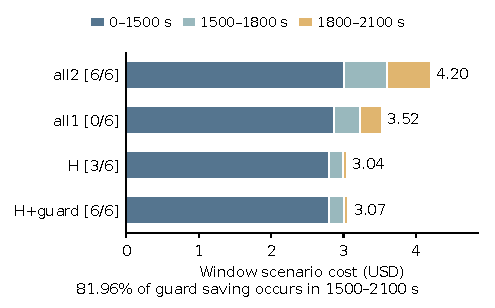
\includegraphics[width=\columnwidth]{figures/v4_w4l_segment_cost.pdf}
\caption{W4-L costs by window-time segment. Bars average three repeats per
window, then weight the two windows equally; brackets give strict passes out
of six. Lower cost in failed runs is not feasible saving. Of the guard's
saving against all2, 81.96\% occurs in the final 600 seconds.}
\label{fig:w4lsegments}
\end{figure}

Thinning reuses observed source windows; intensity was selected by the
registered all2 feasibility gate, not outcome-independent sampling. The result
is therefore load-conditioned, not a new held-out trace. Offline arrivals
continue during $[1500,1800)$, and the back window retains an online arrival
at the closed 1500-second endpoint, so source-window timing and ledger segments
are reported separately. These results do not estimate Azure's production QoS,
required fleet size, model quality, energy use, or bills.
